\subsection{ChatterBot WolfBot}\label{subsec:bot5}

O WolfBot foi desenvolvido em Python com objetivo de executar \emph{querys} do Wolfram Alpha direto no Discord.
Possui o código aberto disponível em \url{https://github.com/Isklar/WolfBot}, além de um breve guia de uso e instalação.
Para realizar uma conversa com o bot, basta entrar no Discord e procurar o servidor que o mantém.
A conversa é unidirecional com o bot respondendo com a execução das consultas enviadas pelo usuário.
Segue um exemplo de conversação:
\subsection{ChatterBot WolfBot}\label{subsec:bot5}

O WolfBot foi desenvolvido em Python com objetivo de executar \emph{querys} do Wolfram Alpha direto no Discord.
Possui o código aberto disponível em \url{https://github.com/Isklar/WolfBot}, além de um breve guia de uso e instalação.
Para realizar uma conversa com o bot, basta entrar no Discord e procurar o servidor que o mantém.
A conversa é unidirecional com o bot respondendo com a execução das consultas enviadas pelo usuário.
Segue um exemplo de conversação:
\subsection{ChatterBot WolfBot}\label{subsec:bot5}

O WolfBot foi desenvolvido em Python com objetivo de executar \emph{querys} do Wolfram Alpha direto no Discord.
Possui o código aberto disponível em \url{https://github.com/Isklar/WolfBot}, além de um breve guia de uso e instalação.
Para realizar uma conversa com o bot, basta entrar no Discord e procurar o servidor que o mantém.
A conversa é unidirecional com o bot respondendo com a execução das consultas enviadas pelo usuário.
Segue um exemplo de conversação:
\subsection{ChatterBot WolfBot}\label{subsec:bot5}

O WolfBot foi desenvolvido em Python com objetivo de executar \emph{querys} do Wolfram Alpha direto no Discord.
Possui o código aberto disponível em \url{https://github.com/Isklar/WolfBot}, além de um breve guia de uso e instalação.
Para realizar uma conversa com o bot, basta entrar no Discord e procurar o servidor que o mantém.
A conversa é unidirecional com o bot respondendo com a execução das consultas enviadas pelo usuário.
Segue um exemplo de conversação:
\input{conversas/bot5}

Depois de um período de testes, percebi que, apesar de realizar o mesmo processo que o chatterbot da seção~\ref{subsec:bot3}, imagens de gráficos não são retornadas. Essa falha pode ser considerada como uma desvantagem ao MathBot, já que ambos propõem o mesmo mecanismo para a mesma plataforma. Por outro lado, as respostas são respondidas como mensagens do bot, e não em imagens (vide a fig.~\ref{fig:bot5_1} abaixo).
\input{img/bot5_1}

O diferencial desse bot está na forma da saída que ele produz. Pode ser toda saída gerada pelo Wolfram Alpha ou apenas uma parte dela, isso é definido de acordo com o comando do usuário. Porém, como esse bot utiliza um sistema externo, a dependência pode ser uma desvantagem pois caso o Wolfram Alpha não esteja funcionando, o bot se tornará inútil.
Abaixo estão listadas algumas melhorias:
\begin{itemize}[noitemsep]
    \item Corrigir a ausência da geração de imagens
    \item Tratar corretamente o erro de entrada do usuário que, ao não passar a \emph{query}, deveria exibir uma mensagem de uso mas o bot responde a última consulta realizada.
    \item Citar o usuário que perguntou na resposta para não ocorrer confusões quando vários usuários estiverem interagindo com o bot
\end{itemize}

Depois de um período de testes, percebi que, apesar de realizar o mesmo processo que o chatterbot da seção~\ref{subsec:bot3}, imagens de gráficos não são retornadas. Essa falha pode ser considerada como uma desvantagem ao MathBot, já que ambos propõem o mesmo mecanismo para a mesma plataforma. Por outro lado, as respostas são respondidas como mensagens do bot, e não em imagens (vide a fig.~\ref{fig:bot5_1} abaixo).
\begin{figure}[h!tbp]
    \centering
    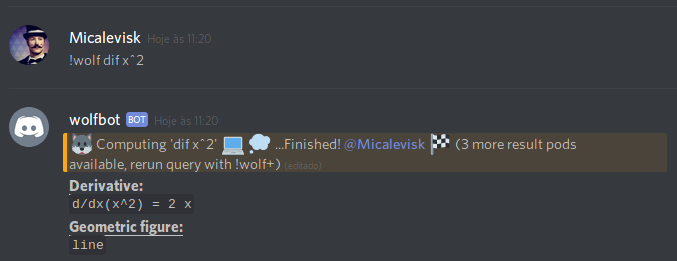
\includegraphics[width=0.9\linewidth]{img/bot5_1.png}
    \caption{Screenshot de uma interação com o WolfBot.}
    \label{fig:bot5_1}
\end{figure}

O diferencial desse bot está na forma da saída que ele produz. Pode ser toda saída gerada pelo Wolfram Alpha ou apenas uma parte dela, isso é definido de acordo com o comando do usuário. Porém, como esse bot utiliza um sistema externo, a dependência pode ser uma desvantagem pois caso o Wolfram Alpha não esteja funcionando, o bot se tornará inútil.
Abaixo estão listadas algumas melhorias:
\begin{itemize}[noitemsep]
    \item Corrigir a ausência da geração de imagens
    \item Tratar corretamente o erro de entrada do usuário que, ao não passar a \emph{query}, deveria exibir uma mensagem de uso mas o bot responde a última consulta realizada.
    \item Citar o usuário que perguntou na resposta para não ocorrer confusões quando vários usuários estiverem interagindo com o bot
\end{itemize}

Depois de um período de testes, percebi que, apesar de realizar o mesmo processo que o chatterbot da seção~\ref{subsec:bot3}, imagens de gráficos não são retornadas. Essa falha pode ser considerada como uma desvantagem ao MathBot, já que ambos propõem o mesmo mecanismo para a mesma plataforma. Por outro lado, as respostas são respondidas como mensagens do bot, e não em imagens (vide a fig.~\ref{fig:bot5_1} abaixo).
\begin{figure}[h!tbp]
    \centering
    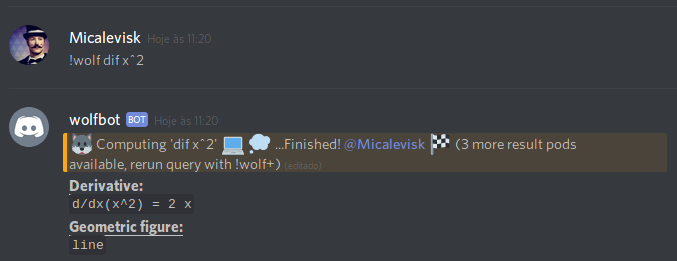
\includegraphics[width=0.9\linewidth]{img/bot5_1.png}
    \caption{Screenshot de uma interação com o WolfBot.}
    \label{fig:bot5_1}
\end{figure}

O diferencial desse bot está na forma da saída que ele produz. Pode ser toda saída gerada pelo Wolfram Alpha ou apenas uma parte dela, isso é definido de acordo com o comando do usuário. Porém, como esse bot utiliza um sistema externo, a dependência pode ser uma desvantagem pois caso o Wolfram Alpha não esteja funcionando, o bot se tornará inútil.
Abaixo estão listadas algumas melhorias:
\begin{itemize}[noitemsep]
    \item Corrigir a ausência da geração de imagens
    \item Tratar corretamente o erro de entrada do usuário que, ao não passar a \emph{query}, deveria exibir uma mensagem de uso mas o bot responde a última consulta realizada.
    \item Citar o usuário que perguntou na resposta para não ocorrer confusões quando vários usuários estiverem interagindo com o bot
\end{itemize}

Depois de um período de testes, percebi que, apesar de realizar o mesmo processo que o chatterbot da seção~\ref{subsec:bot3}, imagens de gráficos não são retornadas. Essa falha pode ser considerada como uma desvantagem ao MathBot, já que ambos propõem o mesmo mecanismo para a mesma plataforma. Por outro lado, as respostas são respondidas como mensagens do bot, e não em imagens (vide a fig.~\ref{fig:bot5_1} abaixo).
\begin{figure}[h!tbp]
    \centering
    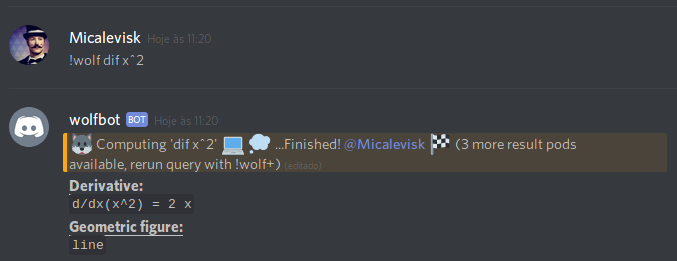
\includegraphics[width=0.9\linewidth]{img/bot5_1.png}
    \caption{Screenshot de uma interação com o WolfBot.}
    \label{fig:bot5_1}
\end{figure}

O diferencial desse bot está na forma da saída que ele produz. Pode ser toda saída gerada pelo Wolfram Alpha ou apenas uma parte dela, isso é definido de acordo com o comando do usuário. Porém, como esse bot utiliza um sistema externo, a dependência pode ser uma desvantagem pois caso o Wolfram Alpha não esteja funcionando, o bot se tornará inútil.
Abaixo estão listadas algumas melhorias:
\begin{itemize}[noitemsep]
    \item Corrigir a ausência da geração de imagens
    \item Tratar corretamente o erro de entrada do usuário que, ao não passar a \emph{query}, deveria exibir uma mensagem de uso mas o bot responde a última consulta realizada.
    \item Citar o usuário que perguntou na resposta para não ocorrer confusões quando vários usuários estiverem interagindo com o bot
\end{itemize}